Objects, being members of many categories, can be called by many names (e.g.,\ a duck can be called \name{duck, bird, animal}, etc.). 
The task of \emph{object naming}---generating not just a formally correct but also an appropriate, \emph{natural} name for an object---is distinct from the closely related tasks of object detection and image classification (see below).
It has been studied in psycholinguistics~(e.g.,~\citealt{Rosch1978}), but has received comparatively little attention in \langvis (\lv) and computational linguistics (CL) research.
We address the following question:\\
\fbox{\parbox{\columnwidth}{\textbf{Q:} Can standard object detection/image classification models (be fine-tuned to) exhibit human-like object naming behavior?}}\\\\
In particular, we test several models for their ability to predict \emph{entry-level names}, i.e., the names people prefer when calling a specific object (e.g.,~\name{bird} in Figure~\ref{fig:duck}, left image).
%% SHORTENING %% We wish to find out, for instance, whether different types of models or training regimes will tend towards different kinds of human-like errors in this regard.
A second contribution of this paper is instrumental: for a proper evaluation we must first augment an existing human object naming dataset (ManyNames, Anonymous, under review) with extensive quality control, the resulting data of which we also describe here.%
\footnote{Data and code for this paper will be made available upon publication.}
\begin{figure}[t]
	\centering
	\small
	\begin{tabular}{p{3cm}p{3cm}}
		\centering
		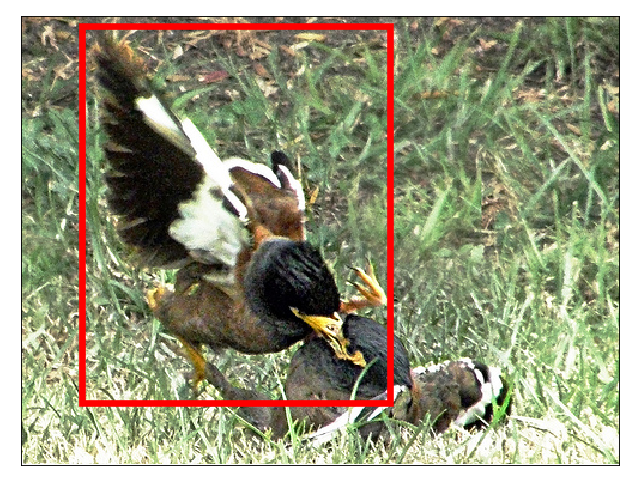
\includegraphics[scale=0.15]{images/2327551_2960743_seed_ambiguous.png} &
		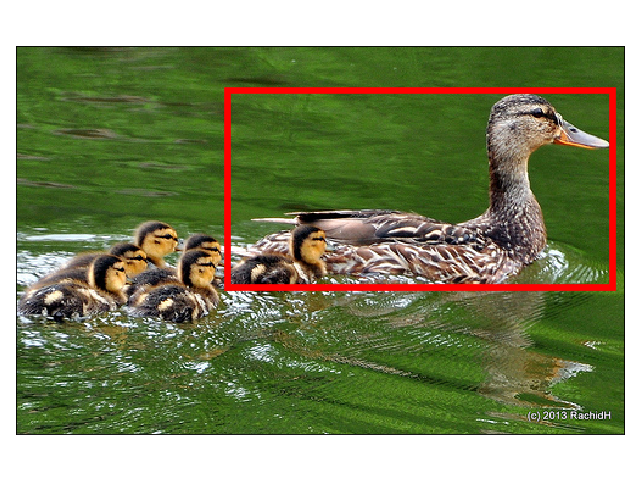
\includegraphics[scale=0.15]{images/2358126_805887_singleton_obj.png}\\
		bird\ (27),  duck\ (8) & duck (33), bird (3)\\
	\end{tabular}
	\caption{Different naming preferences (frequencies) for instances of the same \category \name{duck} in \mn.\label{fig:duck}}
\end{figure}

In \lv, object naming underlies virtually all tasks that model how speakers refer to objects in the world, such as image description or visual question answering.
\lv methods are generally based on object detection or image classification models from computer vision (CV) that were pre-trained towards predicting the single label of each object that is deemed correct by the dataset.
The labels used often seem unintuitive from a human perspective, e.g., some are very basic, natural names (\name{bus}) while others are much more specific (\name{goblet, gyromitra}), cf.\ the label inventory of the ILSVRC challenges \cite{ILSVRC15}.
Pre-training on such labels can enable CV models to learn rich, discriminative visual feature representations which capture fine-grained differences in object appearances (e.g.,\ sharp-pointed vs. slightly pointed). 
But it raises the issue of whether these models could be directly used for more human-like object naming.
% Accordingly, these CV models are assessed by their ability to predict a single, in cases very specific, ground-truth label.

% By contrast, the goal of \lv object naming models is to predict the `natural' name of an object, i.e.,~the name a human could choose for the object instance.
Psycholinguistic studies have found that humans have a preference towards a particular name, defined as the \textit{entry-level name}, when naturally naming an object \cite{rosch1976basic,Rosch1978,jolicoeur1984pictures}. 
However, this research has traditionally focused on \categories and/or their prototypical/schematic depictions (e.g., \citealt{rossion2004revisiting}), as opposed to the situated instances in naturalistic images with which \lv is mostly concerned.
But humans may prefer different names for instances of the same \category (e.g., Figure~\ref{fig:duck}), and even disagree in their choice for the same instance (see also \citealt{graf2016animal}).
%% SHORTENING %% For example, in Figure~\ref{fig:duck} most people (27 out of 36) called the duck on the left \name{bird}, while \name{duck} was strongly preferred for the duck on the right. 

Hence, both the single-ground-truth view of CV models and the category-level approach predominant in psycholinguistics are insufficient for assessing the effectiveness of \lv models for human-like, entry-level object naming.
The ManyNames (MN) dataset was designed to help mend this gap: it consists of names entered by 36~annotators in parallel, for 25K~objects in naturalistic images from \vg~\cite{krishna2016visualgenome}.
However, the annotations of \mn have not been verified to filter out incorrect names or names for the wrong object, a problem that is in some sense the opposite of that posed by the single-ground-truth approach.

Our main contributions are to (i) run the \mn data through a rigorous annotation round to quantify both the adequacy of its names and the types of errors they contain, in order to (ii) test and compare object detection and image classification models at the task of \emph{instance-based, entry-level object naming}. 
More precisely we define entry-level name as follows:\\
%, \mn enables us to define entry-level name as follows:\\
\fbox{\parbox{\columnwidth}{\textbf{Entry-level name:} the most common name given to an object instance according to ManyNames}}\\\\
We evaluate the effectiveness of different models on predicting these entry-level names, and our additional verification annotations enable us to understand the kinds of mistakes the models make (e.g.,~a `wrong' prediction may be a less preferred name as opposed to a true error).
We show that generic object classification models on their own already learn to provide entry-level names for objects, but also that they can transfer-learn on \mn, successfully using pre-trained features from object detection and image classification models to train entry-level naming models. 
%% SHORTENING %% \mw{Remark about the kinds of human errors, just as in the abstract, or some other more interesting teaser?}

%% END OF FILE %%

%Our contributions towards the task of instance-based entry-level naming in \lv and CL research are two-fold:  
%First, we provide data on object naming with real images on a large scale. 
%We take on an empirical notion of entry-level names, and define it on the instance-level, i.e., the name that humans prefer to use when calling a particular object in a real-world image.   
%We extend \mn (under submission), a dataset that provides 36 names for each of 25K objects from \vg~\cite{krishna2016visualgenome}, with information on adequacy and reference of all collected names, which affords rich analysis possibilities. 
%
%Second, we introduce the verified \mn dataset as evaluation data, and provide an extensive analysis of the ability of object detection and classification models to account for entry-level object naming in our dataset. 


\iffalse
%However, when they speak, humans in general name specific \textit{instances} of objects---actually, instances in particular situations and points of view, which may humans have prefer different names for instances of the same \category, and have them even disagree in their choice for the same instance (see also \citealt{graf2016animal}). 


%Accordingly, datasets used for object naming in Psycholinguistics use idealized drawings that correspond more to categories than to instances~\cite{+++++}.
%
%

Despite its relevance in \lv and CL, the challenge of instance-based natural naming has been overseen. 
\lv research that particularly focuses on the prediction of entry-level names is scarce, and existing work has adopted the \category-based concept of entry-level names \cite{Ordonez:2016}. 
Furthermore, existing datasets lack necessary information to make progress in \lv and CL research on this phenomenon. 
\cs{TODO@CS: EVALUATION ISSUE GOES HERE.}
\begin{itemize}
	\item resources developed in CV and \lv can be useful to study object naming. 
	\item However, they provide only one (or a few) name per object \ra no guarantee that it is the entry-level name. (We provide more, to have a robust estimate of entry-level names (as well as data on other possible names). \gbt{actually, maybe move this to the previous part? \ra differences with Psycholing, with CV resources})
	\item object naming has often been conflated with object classification in CV. \gbt{Discuss differences; mention the swan - whatever name it has in wordnet example of ordonez et al?}
	\item a big problem with this approach is that it follows a single-label evaluation. With our data, we show that often model responses are adequate even if they do not correspond to the entry-level name.
	\item we also show that object classification models ``spontaneously'' learn to provide entry-level names for objects
	\item and that it is possible to use \mn to successfully fine-tune existing object detection and classification models to predict entry-level names for objects.
\end{itemize}


This paper seeks to spur \lv and CL research on the problem of \textit{instance-based entry-level object naming}. 

Our contributions are two-fold:  
First, we provide data on object naming with real images on a large scale. 
We take on an empirical notion of entry-level names, and define it on the instance-level, i.e., the name that humans prefer to use when calling a particular object in a real-world image.   
We extend \mn (under submission), a dataset that provides 36 names for each of 25K objects from \vg~\cite{+++}, with information on adequacy and reference of all collected names, which affords rich analysis possibilities. 

\cs{I'll continue from here.}
Second, we introduce the verified \mn dataset as evaluation data that allows XXX. We provide an extensive analysis of the ability of object detection and classification models on the task of predicting the entry-level names in our dataset.


When people talk, they choose particular names for objects, such as \textit{bird} or \textit{duck} for the images in Figure~\ref{fig:duck}.
The task of \textbf{object naming} has been studied in Psycholinguistics~\cite{refs}, \gbt{Which term do you prefer, Psycholing, or CogSci? I don't care. Use same term throughout.} but has not received much attention in Computational Linguistics; we seek to remedy this situation by providing data and modeling results on this phenomenon, and in particular on \textbf{entry-level names}, defined in psycholinguistic research as the preferred name for an object~\cite{rosch1976basic,Rosch1978,jolicoeur1984pictures}: For the left object in the figure, according to our data, the entry-level name is \textit{bird}, and for the right object it is instead \textit{duck}.
%We seek to shed light into how people naturally name objects in real images, and in 


Our contributions are two-fold.
First, we provide data on object naming with real images on a large scale.
We extend \mn (under submission), a dataset that provides 36 names for each of 25K objects from \vg~\cite{+++}, with information on adequacy and reference of all collected names, which affords rich analysis possibilities. 
Our data contain object instances, corresponding more closely to the kind of visual objects that humans typically encounter, and so can potentially shed light on the instance-level factors that affect naming. 

Second, we provide an extensive analysis of the performance of object classification models on the task of predicting the entry-level names in our dataset.

As for the former, note that Psycholinguistic research on entry-level names has focused on categories, as opposed to instances:
When a subcategory is atypical, such as penguins not being very typical birds, this affects their entry-level name (it is common to call a sparrow, but not a penguin, \textit{bird}).
Accordingly, datasets used for object naming in Psycholinguistics use idealized drawings that correspond more to categories than to instances~\cite{+++++}.
However, when they speak, humans in general name specific \textit{instances} of objects ---actually, object instances in particular situations and points of view.
Our data contain object instances, corresponding more closely to the kind of visual objects that humans typically encounter, and so can potentially shed light on the instance-level factors that affect naming.
%Indeed, Psycholinguistic research has typically ignored
% The example shows two instances of the category \textsc{duck}, and when people were asked to name the highlighted object, most ($27$) people called the instance on the left \name{bird}, while \name{duck} was strongly preferred for the right instance. 
%It seems plausible that there are instance-specific factors affecting naming behavior in general.
%, and entry-level names in particular, and our data suggest that this is the case
% gbt: maybe put back a "crucially" somewhere: "Crucially, though, as we will empirically show, human object naming is \textit{instance}-dependent: It depends on the characteristics "
In particular, we validate the notion of entry-level name at the instance level:
For almost 90\% of the 25K objects analyzed, humans showed a preference for a given name (frequency of that name $>50\%$ of the valid responses).

As for the second contribution, \gbt{to be expanded; proposed structure follows; probably here only a summary and a fuller explanation later?}
% allows for an in-depth analysis of naming data as well as of naming models on the task of object naming.
\begin{itemize}
\item resources developed in CV and \lv can be useful to study object naming. 
\item However, they provide only one (or a few) name per object \ra no guarantee that it is the entry-level name. (We provide more, to have a robust estimate of entry-level names (as well as data on other possible names). \gbt{actually, maybe move this to the previous part? \ra differences with Psycholing, with CV resources})
\item object naming has often been conflated with object classification in CV. \gbt{Discuss differences; mention the swan - whatever name it has in wordnet example of ordonez et al?}
\item a big problem with this approach is that it follows a single-label evaluation. With our data, we show that often model responses are adequate even if they do not correspond to the entry-level name.
\item we also show that object classification models ``spontaneously'' learn to provide entry-level names for objects
\item and that it is possible to use \mn to successfully fine-tune existing object detection and classification models to predict entry-level names for objects.
\end{itemize}

\gbt{Below is the old text. I factored out the entry-level aspects in the previous paragraph. It should be removed from this second part.}

Objects, being members of many categories, can be called by many names (e.g.,\ a duck can be called \name{duck, bird, animal} etc.). 
In \langvis research (\lv), the choice of a particular name for an object is a ubiquitous problem---it underlies virtually all tasks that model how speakers use language to refer to objects in the world, such as image description, visual question answering, referring expression generation, etc. 
%
\lv methods are generally based on object detection or image classification models (or the visual features extracted from them) that were pre-trained towards predicting the single correct label of objects. 
The set of labels are often determined rather arbitrarily---it may contain very specific (e.g.,\ \name{goblet, gyromitra}) as well as "basic-level" labels (e.g., \name{bus}; cf.\ the label inventory of the ILSVRC challenges; \citealt{ILSVRC15}). 

This pre-training strategy has its justification in that computer vision models can learn rich, discriminative visual feature representations which capture fine-grained differences in object appearances (e.g.,\ sharp--pointed vs. slightly pointed). 
It is, however, different from predicting the natural name of an object, 
because, as has been found in numerous studies in psychology, humans have a preference towards a particular name (\textit{entry-level name}, e.g.,\ \name{duck}) when naturally calling an object  \cite{rosch1976basic,Rosch1978,jolicoeur1984pictures}. 
Entry-level names have hereby usually been considered to be an attribute of concrete \textit{concepts} (e.g.,\ penguin, duck), where the choice of a concept's entry-level name depends on factors such as its typicality with respect to its basic-level category (bird). \cs{Need to check Jolicoeur and their experiments} 
Crucially, though, as we will empirically show, human object naming is \textit{instance}-dependent---contextual visual features may humans have prefer different names for object instances of the same concrete concept, and have them even disagree in their choice for the same instance (see also \citealt{graf2016animal}). 
For example, Figure~\ref{fig:duck} shows two instances of the concept duck, and when people were asked to name the highlighted object, most ($27$) people called the instance on the left \name{bird}, while \name{duck} was strongly preferred for the right instance. 

Despite its relevance in \lv, the challenge of instance-based natural naming has been overseen, and most \lv datasets not necessarily provide enough information to make progress on the problem of modeling natural object naming (they only provide very few names). 
Research that particularly focuses on the prediction of entry-level names is scarce, and existing work has adopted the view that (i) entry-level names arise on the conceptual level, and (ii) developed specialized methods \cite{Ordonez:2016}. 
%To our knowledge, work that gives systematic insights into the ability of standard object recognition models to account for natural object naming, and in how far simple \cs{straightfoward?} re-training or transfer learning can increase this ability, is lacking. 
%

In this paper, we seek an understanding of the notion of entry-level names of instances of real-world objects in images, and to give systematic insights into the problem of retraining or fine-tuning object detection models (and features in transfer learning) such that they capture a natural vocabulary and account for linguistic preferences in naming. %, i.e.,\ the name that humans naturally prefer to call an object.  
Specifically, and in contrast to previous works, we 
(i) take on an empirical notion of entry-level names, and define it on the instance-level, i.e., the name that humans prefer to use when calling a particular object in a real-world image.   
(ii) We examine in how far standard models in computer vision, namely object detection and image classification models, do learn entry-level naming by being trained on images labeled with rather \textit{\arbitrary} (as opposed to entry-level) object names. \cs{add sth based on results - how to fine-tune or whether it's possible to fine-tune; how readily available they are to be used for transfer learning, the standard method in \lv}

We use \mn, a new dataset of real-world images, built on top of \vg, which provides an excellent resource for our study, since it was annotated with a large number\ $(36)$ of object names by means of a crowdsourcing study.

Our contributions are: 
(i) We present our extension of the \mn dataset that augments all collected object names with verification information, which allows an in-depth analysis of naming models on the task of object naming. 
(ii) Theoretical:
(a) We show that entry-level names should be derived on the instance-level as opposed to the XXX level \cs{(TO SHOW: entry-level names are different for the same "class" @Sina or @Matthijs?) (contrast to psychological studies)}
(b) We need many name annotations to derive the entry-level name (contrast to few annotations in L+V and computer vision; \cs{TO SHOW: entry-level name of an instance varies depending on the number of annotations/instance)}
(iii) Technical:
(a) Object detectors trained on "\arbitrary" natural object names do learn entry-level names to some extend (as expected: they learn the shared features leading to entry-level \cs{-- can we show that mistakes are rather class-based? i.e., tendency towards a certain name for each class?)}
(b) To predict entry-level names without annotating a huge amount of training examples, it is possible to fine-tune (iii) on \mn. We show that \cs{(say something about mistakes not made anymore). }

\fi
%%% Local Variables:
%%% mode: latex
%%% TeX-master: "acl2020_main"
%%% End:
